In this section we describe our experimental evaluation, discussing
the performance indicators used to compare different strategies, the
simulator developed and used to emulate the behavior of
brownout-compliant replicas driven by the load-balancer and our case
studies.

\subsection{Performance indicators}

Performance measures are necessary to objectively compare different
algorithms. While our first performance indicator is clearly defined
as the \textbf{percentage $\%_{on}$} of the total requests served with
the optional content enabled, we also would like to introduce some
other performance metrics to compare the implemented load-balancing
techniques.

Another metric considered for this study is the \textbf{user-perceived
  stability $\sigma_u$}~\cite{GeograficalSASO}. This metric refers to
the variation of perfomance as observed by the users, and it is
measured as the standard deviation of the vector of response
times. Its purpose is to measure the ability of the replicas to
respond timely to the client requests. The entire brownout framework
aims at stabilizing the response times, therefore it should achieve
low user-perceived stability, irregardless of the presence of the
load-balancer. However, the load-balancing algorithm clearly
influences the perceived latencies, therefore it is logical to check
whether the newly developed algorithms achieve a better perceived
stability with respect to the classical ones. Together with the value
of the user-perceived stability, we also report the \textbf{average
  response time $\mu_u$} to distinguish between algorithms that
achieve a low response time with possibly high fluctuations from
solutions that achieve a higher but more stable response time.

\subsection{Simulator}

To test our load-balancing strategies, together with existing state 
of the art solutions, we implemented a simulator for brownout-compliant 
applications. In the simulator, it is very easy to plug-in new 
load-balancing algorithms. The simulator is based on the concepts of 
\emph{Client},  \emph{Request}, \emph{LoadBalancer}, \emph{Replica} 
and \emph{Link}.

When a new client is defined, it can behave according to the open-loop 
client model, where it simply issues a certain number of unrelated
requests (as it is true for clients that respect the Markovian assumption),
or according to che closed-loop one. Closed-loop clients issue a request
and wait for the response, whenever they receive the response they think
for some time and subsequently continue using the application with another
request. While this second model is more realistic, the first one is still
useful to simulate the behavior of the mass. The simulator implements
both of them, to allow for complete test.

Requests are received by the load-balancer, that directs them towards
different replicas. The load-balancer can work on a per-request basis or
based on weights. The first case is used to simulate policies like
Round Robin, Random, Shortest Queue First and so on, that do not rely on
the concept of weights. The weighted load-balancer is used to simulate the
strategies proposed in this paper, as well as state of the art solutions
like the Weighted Round Robin. 

Each replica simulates the computation necessary to serve the request
and chooses if it should be executed with or without the optional components
activated. Service times depend on that. The replicas are also executing
an internal control loop to select their control variables, the probability
of executing the optional components. Details on how the interal control 
loops are realized can be found on~\cite{cloudish-tr}.

Finally, there are network links connecting the load-balancer and the
replicas. These link are part of the simulator, to study the effect of
network delays in communicating the necessary feedback information for the
load-balancer execution.

The simulator receives as input a \emph{Scenario}, which describes what
can happen during the simulation. The scenario definition supports the
insertion of new clients and the removal of existing ones. It also allows
to turn on and off replicas at specific times during the execution and to
change the service times for every replica, both for the optional
components and for the mandatory ones. This simulates a change in the
amount of resources given to the machine hosting the replica and it is
based on the assumption that these changes are unpredictable and can
happen at the architecture level, for example due to the cloud provider
co-locating more applications onto the same physical hardware, therefore
reducing their computation capability.

With the scenarios, it is very easy to simulate different working
conditions and to have a complete overview of the changes that might
happen during the load-balancing and replica execution. In the following,
we describe two sets of experiments conducted to compare the load-balancing
strategies when subject to different execution conditions.

\subsection{Reacting to clients behavior}

The aim of this first test is to evaluate the performance of
different algorithms when new clients are arriving and some other clients
disconnect.

We present an experiment where the infrastructure is composed by four 
replicas. The fist replica is the fastest and requires $0.05$ seconds to 
serve a request with the optional components, while only $0.005$ are 
necessary to produce the answer without optional components. The second 
replica is slower and takes $0.25$ to produce a full request and $0.025$ 
seconds to produce the mandatory content. The third and fourth replicas 
are even slower, taking $0.5$ seconds for the full content and $0.05$ for 
the mandatory content only.

Clients are added according to the closed-loop model. $50$ clients are
accessing the system at the beginning of the simulation, time $0$ and $10$ of 
them are removed after $200$ seconds. At time $400$, $25$ more clients
access the application and $25$ more arrives again at $600$ seconds. 
$40$ clients and the simulation is ended at time $1000$.

\begin{figure}
\centering
\begin{tikzpicture}[scale=0.95,transform shape]
\pgfplotsset{width=0.6\columnwidth,height=3.2cm}
\pgfplotsset{filter discard warning=false}
\pgfplotsset{grid style={dashed}}
\begin{groupplot}
[
group style={
       group name=my plots,
       group size=2 by 11,
       xlabels at=edge bottom,
       xticklabels at=edge bottom,
       ylabels at=edge left,
       yticklabels at=edge left,
       vertical sep=0.25cm,
       horizontal sep=0.5cm},
xmajorgrids,
ymajorgrids,
xlabel={$t$ [sec]},
xmin=0,xmax=1000,
ymin=-0.05,
ymax= 1.05,
scaled ticks=false,
xtick={0,200,...,1000},
xticklabel style={font=\footnotesize},
yticklabel style={font=\footnotesize},
%ytick align=outside,
%xtick align=outside,
]

% index variable
% 0     time
% 1     weight replica 1
% 2     weight replica 2
% 3     weight replica 3
% 4     weight replica 4
% 5     dimmer replica 1
% 6     dimmer replica 2
% 7     dimmer replica 3
% 8     dimmer replica 4
% 9     average latency replica 1
% 10    average latency replica 2
% 11    average latency replica 3
% 12    average latency replica 4
% 13    max latency or nan replica 1
% 14    max latency or nan replica 2
% 15    max latency or nan replica 3
% 16    max latency or nan replica 4
% 17    total number of served requests
% 18    total number of served requests with optional content
% 19    actual weight replica 1
% 20    actual weight replica 2
% 21    actual weight replica 3
% 22    actual weight replica 4


%% 1st row
\nextgroupplot[
title={$w$},
ylabel={EPBH}, % equal-thetas
]

\addplot[black] table[x index=0,y index=19,col sep=comma,each nth point=1]{img/clientchanges-full/equal-thetas/sim-lb.csv};
\addplot[blue]  table[x index=0,y index=20,col sep=comma,each nth point=1]{img/clientchanges-full/equal-thetas/sim-lb.csv};
\addplot[green] table[x index=0,y index=21,col sep=comma,each nth point=1]{img/clientchanges-full/equal-thetas/sim-lb.csv};
\addplot[red]   table[x index=0,y index=22,col sep=comma,each nth point=1]{img/clientchanges-full/equal-thetas/sim-lb.csv};

\nextgroupplot[
title={$\theta$},
]

\addplot[black] table[x index=0,y index=5,col sep=comma,each nth point=1]{img/clientchanges-full/equal-thetas/sim-lb.csv};
\addplot[blue]  table[x index=0,y index=6,col sep=comma,each nth point=1]{img/clientchanges-full/equal-thetas/sim-lb.csv};
\addplot[green] table[x index=0,y index=7,col sep=comma,each nth point=1]{img/clientchanges-full/equal-thetas/sim-lb.csv};
\addplot[red]   table[x index=0,y index=8,col sep=comma,each nth point=1]{img/clientchanges-full/equal-thetas/sim-lb.csv};


%% 2nd row
\nextgroupplot[
ylabel={VPBH}, % theta-diff-plus
]

\addplot[black] table[x index=0,y index=19,col sep=comma,each nth point=1]{img/clientchanges-full/theta-diff-plus/sim-lb.csv};
\addplot[blue]  table[x index=0,y index=20,col sep=comma,each nth point=1]{img/clientchanges-full/theta-diff-plus/sim-lb.csv};
\addplot[green] table[x index=0,y index=21,col sep=comma,each nth point=1]{img/clientchanges-full/theta-diff-plus/sim-lb.csv};
\addplot[red]   table[x index=0,y index=22,col sep=comma,each nth point=1]{img/clientchanges-full/theta-diff-plus/sim-lb.csv};

\nextgroupplot[]

\addplot[black] table[x index=0,y index=5,col sep=comma,each nth point=1]{img/clientchanges-full/theta-diff-plus/sim-lb.csv};
\addplot[blue]  table[x index=0,y index=6,col sep=comma,each nth point=1]{img/clientchanges-full/theta-diff-plus/sim-lb.csv};
\addplot[green] table[x index=0,y index=7,col sep=comma,each nth point=1]{img/clientchanges-full/theta-diff-plus/sim-lb.csv};
\addplot[red]   table[x index=0,y index=8,col sep=comma,each nth point=1]{img/clientchanges-full/theta-diff-plus/sim-lb.csv};

%% 3rd row
\nextgroupplot[
ylabel={OBLB}, % Optimization
]

\addplot[black] table[x index=0,y index=19,col sep=comma,each nth point=1]{img/clientchanges-full/optimization/sim-lb.csv};
\addplot[blue]  table[x index=0,y index=20,col sep=comma,each nth point=1]{img/clientchanges-full/optimization/sim-lb.csv};
\addplot[green] table[x index=0,y index=21,col sep=comma,each nth point=1]{img/clientchanges-full/optimization/sim-lb.csv};
\addplot[red]   table[x index=0,y index=22,col sep=comma,each nth point=1]{img/clientchanges-full/optimization/sim-lb.csv};

\nextgroupplot[]

\addplot[black] table[x index=0,y index=5,col sep=comma,each nth point=1]{img/clientchanges-full/optimization/sim-lb.csv};
\addplot[blue]  table[x index=0,y index=6,col sep=comma,each nth point=1]{img/clientchanges-full/optimization/sim-lb.csv};
\addplot[green] table[x index=0,y index=7,col sep=comma,each nth point=1]{img/clientchanges-full/optimization/sim-lb.csv};
\addplot[red]   table[x index=0,y index=8,col sep=comma,each nth point=1]{img/clientchanges-full/optimization/sim-lb.csv};

%% 4th row
\nextgroupplot[
ylabel={SQF},
]

\addplot[black] table[x index=0,y index=19,col sep=comma,each nth point=1]{img/clientchanges-full/SQF/sim-lb.csv};
\addplot[blue]  table[x index=0,y index=20,col sep=comma,each nth point=1]{img/clientchanges-full/SQF/sim-lb.csv};
\addplot[green] table[x index=0,y index=21,col sep=comma,each nth point=1]{img/clientchanges-full/SQF/sim-lb.csv};
\addplot[red]   table[x index=0,y index=22,col sep=comma,each nth point=1]{img/clientchanges-full/SQF/sim-lb.csv};

\nextgroupplot[]

\addplot[black] table[x index=0,y index=5,col sep=comma,each nth point=1]{img/clientchanges-full/SQF/sim-lb.csv};
\addplot[blue]  table[x index=0,y index=6,col sep=comma,each nth point=1]{img/clientchanges-full/SQF/sim-lb.csv};
\addplot[green] table[x index=0,y index=7,col sep=comma,each nth point=1]{img/clientchanges-full/SQF/sim-lb.csv};
\addplot[red]   table[x index=0,y index=8,col sep=comma,each nth point=1]{img/clientchanges-full/SQF/sim-lb.csv};

%% 5th row
\nextgroupplot[
ylabel={FRF-EWMA},
]

\addplot[black] table[x index=0,y index=19,col sep=comma,each nth point=1]{img/clientchanges-full/FRF-EWMA/sim-lb.csv};
\addplot[blue]  table[x index=0,y index=20,col sep=comma,each nth point=1]{img/clientchanges-full/FRF-EWMA/sim-lb.csv};
\addplot[green] table[x index=0,y index=21,col sep=comma,each nth point=1]{img/clientchanges-full/FRF-EWMA/sim-lb.csv};
\addplot[red]   table[x index=0,y index=22,col sep=comma,each nth point=1]{img/clientchanges-full/FRF-EWMA/sim-lb.csv};

\nextgroupplot[]

\addplot[black] table[x index=0,y index=5,col sep=comma,each nth point=1]{img/clientchanges-full/FRF-EWMA/sim-lb.csv};
\addplot[blue]  table[x index=0,y index=6,col sep=comma,each nth point=1]{img/clientchanges-full/FRF-EWMA/sim-lb.csv};
\addplot[green] table[x index=0,y index=7,col sep=comma,each nth point=1]{img/clientchanges-full/FRF-EWMA/sim-lb.csv};
\addplot[red]   table[x index=0,y index=8,col sep=comma,each nth point=1]{img/clientchanges-full/FRF-EWMA/sim-lb.csv};

%% 6th row
\nextgroupplot[
ylabel={2RC},
]

\addplot[black] table[x index=0,y index=19,col sep=comma,each nth point=1]{img/clientchanges-full/2RC/sim-lb.csv};
\addplot[blue]  table[x index=0,y index=20,col sep=comma,each nth point=1]{img/clientchanges-full/2RC/sim-lb.csv};
\addplot[green] table[x index=0,y index=21,col sep=comma,each nth point=1]{img/clientchanges-full/2RC/sim-lb.csv};
\addplot[red]   table[x index=0,y index=22,col sep=comma,each nth point=1]{img/clientchanges-full/2RC/sim-lb.csv};

\nextgroupplot[]

\addplot[black] table[x index=0,y index=5,col sep=comma,each nth point=1]{img/clientchanges-full/2RC/sim-lb.csv};
\addplot[blue]  table[x index=0,y index=6,col sep=comma,each nth point=1]{img/clientchanges-full/2RC/sim-lb.csv};
\addplot[green] table[x index=0,y index=7,col sep=comma,each nth point=1]{img/clientchanges-full/2RC/sim-lb.csv};
\addplot[red]   table[x index=0,y index=8,col sep=comma,each nth point=1]{img/clientchanges-full/2RC/sim-lb.csv};

%% 7th row
\nextgroupplot[
ylabel={FRF},
]

\addplot[black] table[x index=0,y index=19,col sep=comma,each nth point=1]{img/clientchanges-full/FRF/sim-lb.csv};
\addplot[blue]  table[x index=0,y index=20,col sep=comma,each nth point=1]{img/clientchanges-full/FRF/sim-lb.csv};
\addplot[green] table[x index=0,y index=21,col sep=comma,each nth point=1]{img/clientchanges-full/FRF/sim-lb.csv};
\addplot[red]   table[x index=0,y index=22,col sep=comma,each nth point=1]{img/clientchanges-full/FRF/sim-lb.csv};

\nextgroupplot[]

\addplot[black] table[x index=0,y index=5,col sep=comma,each nth point=1]{img/clientchanges-full/FRF/sim-lb.csv};
\addplot[blue]  table[x index=0,y index=6,col sep=comma,each nth point=1]{img/clientchanges-full/FRF/sim-lb.csv};
\addplot[green] table[x index=0,y index=7,col sep=comma,each nth point=1]{img/clientchanges-full/FRF/sim-lb.csv};
\addplot[red]   table[x index=0,y index=8,col sep=comma,each nth point=1]{img/clientchanges-full/FRF/sim-lb.csv};

%% 8th row
\nextgroupplot[
ylabel={Random},
]

\addplot[black] table[x index=0,y index=19,col sep=comma,each nth point=1]{img/clientchanges-full/random/sim-lb.csv};
\addplot[blue]  table[x index=0,y index=20,col sep=comma,each nth point=1]{img/clientchanges-full/random/sim-lb.csv};
\addplot[green] table[x index=0,y index=21,col sep=comma,each nth point=1]{img/clientchanges-full/random/sim-lb.csv};
\addplot[red]   table[x index=0,y index=22,col sep=comma,each nth point=1]{img/clientchanges-full/random/sim-lb.csv};

\nextgroupplot[]

\addplot[black] table[x index=0,y index=5,col sep=comma,each nth point=1]{img/clientchanges-full/random/sim-lb.csv};
\addplot[blue]  table[x index=0,y index=6,col sep=comma,each nth point=1]{img/clientchanges-full/random/sim-lb.csv};
\addplot[green] table[x index=0,y index=7,col sep=comma,each nth point=1]{img/clientchanges-full/random/sim-lb.csv};
\addplot[red]   table[x index=0,y index=8,col sep=comma,each nth point=1]{img/clientchanges-full/random/sim-lb.csv};

%% 9th row
\nextgroupplot[
ylabel={RR},
]

\addplot[black] table[x index=0,y index=19,col sep=comma,each nth point=1]{img/clientchanges-full/RR/sim-lb.csv};
\addplot[blue]  table[x index=0,y index=20,col sep=comma,each nth point=1]{img/clientchanges-full/RR/sim-lb.csv};
\addplot[green] table[x index=0,y index=21,col sep=comma,each nth point=1]{img/clientchanges-full/RR/sim-lb.csv};
\addplot[red]   table[x index=0,y index=22,col sep=comma,each nth point=1]{img/clientchanges-full/RR/sim-lb.csv};

\nextgroupplot[]

\addplot[black] table[x index=0,y index=5,col sep=comma,each nth point=1]{img/clientchanges-full/RR/sim-lb.csv};
\addplot[blue]  table[x index=0,y index=6,col sep=comma,each nth point=1]{img/clientchanges-full/RR/sim-lb.csv};
\addplot[green] table[x index=0,y index=7,col sep=comma,each nth point=1]{img/clientchanges-full/RR/sim-lb.csv};
\addplot[red]   table[x index=0,y index=8,col sep=comma,each nth point=1]{img/clientchanges-full/RR/sim-lb.csv};

%% 10th row
\nextgroupplot[
ylabel={Predictive},
]

\addplot[black] table[x index=0,y index=19,col sep=comma,each nth point=1]{img/clientchanges-full/predictive/sim-lb.csv};
\addplot[blue]  table[x index=0,y index=20,col sep=comma,each nth point=1]{img/clientchanges-full/predictive/sim-lb.csv};
\addplot[green] table[x index=0,y index=21,col sep=comma,each nth point=1]{img/clientchanges-full/predictive/sim-lb.csv};
\addplot[red]   table[x index=0,y index=22,col sep=comma,each nth point=1]{img/clientchanges-full/predictive/sim-lb.csv};

\nextgroupplot[]

\addplot[black] table[x index=0,y index=5,col sep=comma,each nth point=1]{img/clientchanges-full/predictive/sim-lb.csv};
\addplot[blue]  table[x index=0,y index=6,col sep=comma,each nth point=1]{img/clientchanges-full/predictive/sim-lb.csv};
\addplot[green] table[x index=0,y index=7,col sep=comma,each nth point=1]{img/clientchanges-full/predictive/sim-lb.csv};
\addplot[red]   table[x index=0,y index=8,col sep=comma,each nth point=1]{img/clientchanges-full/predictive/sim-lb.csv};

%% 11th row
\nextgroupplot[
ylabel={Weighted-RR},
]

\addplot[black] table[x index=0,y index=19,col sep=comma,each nth point=1]{img/clientchanges-full/weighted-RR/sim-lb.csv};
\addplot[blue]  table[x index=0,y index=20,col sep=comma,each nth point=1]{img/clientchanges-full/weighted-RR/sim-lb.csv};
\addplot[green] table[x index=0,y index=21,col sep=comma,each nth point=1]{img/clientchanges-full/weighted-RR/sim-lb.csv};
\addplot[red]   table[x index=0,y index=22,col sep=comma,each nth point=1]{img/clientchanges-full/weighted-RR/sim-lb.csv};

\nextgroupplot[]

\addplot[black] table[x index=0,y index=5,col sep=comma,each nth point=1]{img/clientchanges-full/weighted-RR/sim-lb.csv};
\addplot[blue]  table[x index=0,y index=6,col sep=comma,each nth point=1]{img/clientchanges-full/weighted-RR/sim-lb.csv};
\addplot[green] table[x index=0,y index=7,col sep=comma,each nth point=1]{img/clientchanges-full/weighted-RR/sim-lb.csv};
\addplot[red]   table[x index=0,y index=8,col sep=comma,each nth point=1]{img/clientchanges-full/weighted-RR/sim-lb.csv};

\end{groupplot}

\end{tikzpicture}


\caption{Results of a simulation with four replicas and clients entering
and leaving the system at different times. The left column shows the
effective weights computed by the load-balancing policies while the
right column shows the control variables for each replica. The first
replica is depicted in black solid lines, the second replica is shown
in blue dashed lines, the third replica in red dotted lines.}
\label{fig:clientchanges-full}
\end{figure}

\begin{figure}
\centering
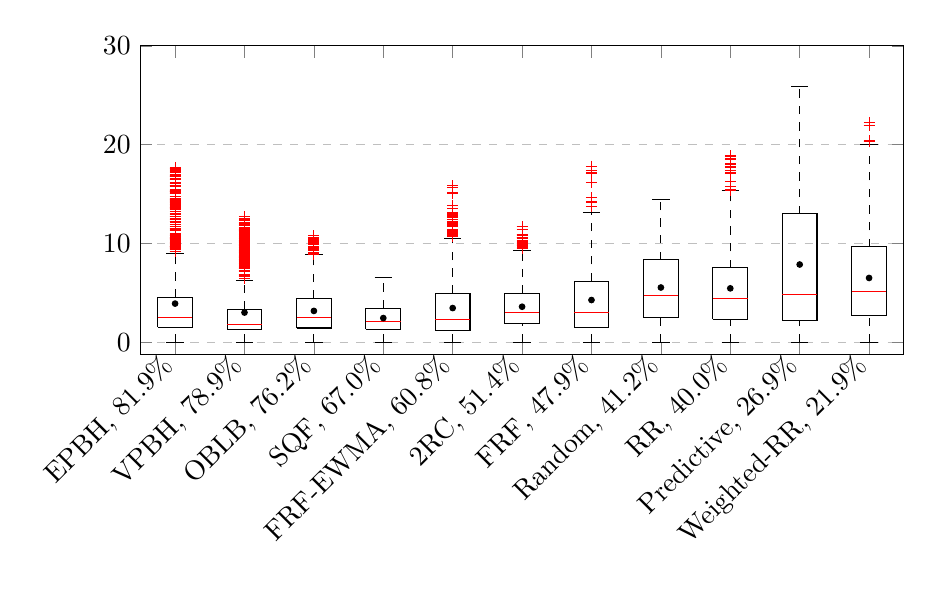
\begin{tikzpicture}[scale=1,transform shape]
\pgfplotsset{grid style={dashed}}
\begin{axis}[%
width=0.93\columnwidth,
height=5.5cm,
xmin=0.5, 
xmax=11.5,
ymin=-1.2, 
ymax=30,
xlabel style = {center},
xtick={1,2,3,4,5,6,7,8,9,10,11,12},
xticklabels={%
{EPBH, $81.9\%$},%
{VPBH, $78.9\%$},%
{OBLB, $76.2\%$},%
{SQF, $67.0\%$},%
{FRF-EWMA, $60.8\%$},%
{2RC, $51.4\%$},%
{FRF, $47.9\%$},%
{Random, $41.2\%$},%
{RR, $40.0\%$},%
{Predictive, $26.9\%$},%
{Weighted-RR, $21.9\%$}%
},
x tick label style={rotate=45, anchor=east},
ymajorgrids,
]
\addplot [
color=black,
dashed
]
coordinates{
 (1,4.57617)(1,9.02788) 
};

\addplot [
color=black,
dashed
]
coordinates{
 (2,3.34152)(2,6.26943) 
};

\addplot [
color=black,
dashed
]
coordinates{
 (3,4.43125)(3,8.86237) 
};

\addplot [
color=black,
dashed
]
coordinates{
 (4,3.465)(4,6.58852) 
};

\addplot [
color=black,
dashed
]
coordinates{
 (5,4.97803)(5,10.5269) 
};

\addplot [
color=black,
dashed
]
coordinates{
 (6,4.92883)(6,9.33183) 
};

\addplot [
color=black,
dashed
]
coordinates{
 (7,6.21138)(7,13.1455) 
};

\addplot [
color=black,
dashed
]
coordinates{
 (8,8.35872)(8,14.4421) 
};

\addplot [
color=black,
dashed
]
coordinates{
 (9,7.54385)(9,15.3635) 
};

\addplot [
color=black,
dashed
]
coordinates{
 (10,13.0111)(10,25.8548) 
};

\addplot [
color=black,
dashed
]
coordinates{
 (11,9.66816)(11,19.9898) 
};

\addplot [
color=black,
dashed
]
coordinates{
 (1,0)(1,1.53656) 
};

\addplot [
color=black,
dashed
]
coordinates{
 (2,0)(2,1.32854) 
};

\addplot [
color=black,
dashed
]
coordinates{
 (3,0)(3,1.4642) 
};

\addplot [
color=black,
dashed
]
coordinates{
 (4,0)(4,1.33472) 
};

\addplot [
color=black,
dashed
]
coordinates{
 (5,0)(5,1.23414) 
};

\addplot [
color=black,
dashed
]
coordinates{
 (6,0)(6,1.91124) 
};

\addplot [
color=black,
dashed
]
coordinates{
 (7,0)(7,1.54043) 
};

\addplot [
color=black,
dashed
]
coordinates{
 (8,0)(8,2.48405) 
};

\addplot [
color=black,
dashed
]
coordinates{
 (9,0)(9,2.32885) 
};

\addplot [
color=black,
dashed
]
coordinates{
 (10,0)(10,2.24439) 
};

\addplot [
color=black,
dashed
]
coordinates{
 (11,0)(11,2.69095) 
};

\addplot [
color=black,
solid
]
coordinates{
 (0.875,9.02788)(1.125,9.02788) 
};

\addplot [
color=black,
solid
]
coordinates{
 (1.875,6.26943)(2.125,6.26943) 
};

\addplot [
color=black,
solid
]
coordinates{
 (2.875,8.86237)(3.125,8.86237) 
};

\addplot [
color=black,
solid
]
coordinates{
 (3.875,6.58852)(4.125,6.58852) 
};

\addplot [
color=black,
solid
]
coordinates{
 (4.875,10.5269)(5.125,10.5269) 
};

\addplot [
color=black,
solid
]
coordinates{
 (5.875,9.33183)(6.125,9.33183) 
};

\addplot [
color=black,
solid
]
coordinates{
 (6.875,13.1455)(7.125,13.1455) 
};

\addplot [
color=black,
solid
]
coordinates{
 (7.875,14.4421)(8.125,14.4421) 
};

\addplot [
color=black,
solid
]
coordinates{
 (8.875,15.3635)(9.125,15.3635) 
};

\addplot [
color=black,
solid
]
coordinates{
 (9.875,25.8548)(10.125,25.8548) 
};

\addplot [
color=black,
solid
]
coordinates{
 (10.875,19.9898)(11.125,19.9898) 
};

\addplot [
color=black,
solid
]
coordinates{
 (0.875,0)(1.125,0) 
};

\addplot [
color=black,
solid
]
coordinates{
 (1.875,0)(2.125,0) 
};

\addplot [
color=black,
solid
]
coordinates{
 (2.875,0)(3.125,0) 
};

\addplot [
color=black,
solid
]
coordinates{
 (3.875,0)(4.125,0) 
};

\addplot [
color=black,
solid
]
coordinates{
 (4.875,0)(5.125,0) 
};

\addplot [
color=black,
solid
]
coordinates{
 (5.875,0)(6.125,0) 
};

\addplot [
color=black,
solid
]
coordinates{
 (6.875,0)(7.125,0) 
};

\addplot [
color=black,
solid
]
coordinates{
 (7.875,0)(8.125,0) 
};

\addplot [
color=black,
solid
]
coordinates{
 (8.875,0)(9.125,0) 
};

\addplot [
color=black,
solid
]
coordinates{
 (9.875,0)(10.125,0) 
};

\addplot [
color=black,
solid
]
coordinates{
 (10.875,0)(11.125,0) 
};

\addplot [
color=black,
solid
]
coordinates{
 (0.75,1.53656)(0.75,4.57617)(1.25,4.57617)(1.25,1.53656)(0.75,1.53656) 
};

\addplot [
color=black,
solid
]
coordinates{
 (1.75,1.32854)(1.75,3.34152)(2.25,3.34152)(2.25,1.32854)(1.75,1.32854) 
};

\addplot [
color=black,
solid
]
coordinates{
 (2.75,1.4642)(2.75,4.43125)(3.25,4.43125)(3.25,1.4642)(2.75,1.4642) 
};

\addplot [
color=black,
solid
]
coordinates{
 (3.75,1.33472)(3.75,3.465)(4.25,3.465)(4.25,1.33472)(3.75,1.33472) 
};

\addplot [
color=black,
solid
]
coordinates{
 (4.75,1.23414)(4.75,4.97803)(5.25,4.97803)(5.25,1.23414)(4.75,1.23414) 
};

\addplot [
color=black,
solid
]
coordinates{
 (5.75,1.91124)(5.75,4.92883)(6.25,4.92883)(6.25,1.91124)(5.75,1.91124) 
};

\addplot [
color=black,
solid
]
coordinates{
 (6.75,1.54043)(6.75,6.21138)(7.25,6.21138)(7.25,1.54043)(6.75,1.54043) 
};

\addplot [
color=black,
solid
]
coordinates{
 (7.75,2.48405)(7.75,8.35872)(8.25,8.35872)(8.25,2.48405)(7.75,2.48405) 
};

\addplot [
color=black,
solid
]
coordinates{
 (8.75,2.32885)(8.75,7.54385)(9.25,7.54385)(9.25,2.32885)(8.75,2.32885) 
};

\addplot [
color=black,
solid
]
coordinates{
 (9.75,2.24439)(9.75,13.0111)(10.25,13.0111)(10.25,2.24439)(9.75,2.24439) 
};

\addplot [
color=black,
solid
]
coordinates{
 (10.75,2.69095)(10.75,9.66816)(11.25,9.66816)(11.25,2.69095)(10.75,2.69095) 
};

\addplot [
color=red,
solid
]
coordinates{
 (0.75,2.5132)(1.25,2.5132) 
};

\addplot [
color=red,
solid
]
coordinates{
 (1.75,1.85185)(2.25,1.85185) 
};

\addplot [
color=red,
solid
]
coordinates{
 (2.75,2.53327)(3.25,2.53327) 
};

\addplot [
color=red,
solid
]
coordinates{
 (3.75,2.11353)(4.25,2.11353) 
};

\addplot [
color=red,
solid
]
coordinates{
 (4.75,2.33437)(5.25,2.33437) 
};

\addplot [
color=red,
solid
]
coordinates{
 (5.75,3.04626)(6.25,3.04626) 
};

\addplot [
color=red,
solid
]
coordinates{
 (6.75,3.07519)(7.25,3.07519) 
};

\addplot [
color=red,
solid
]
coordinates{
 (7.75,4.77691)(8.25,4.77691) 
};

\addplot [
color=red,
solid
]
coordinates{
 (8.75,4.41638)(9.25,4.41638) 
};

\addplot [
color=red,
solid
]
coordinates{
 (9.75,4.88217)(10.25,4.88217) 
};

\addplot [
color=red,
solid
]
coordinates{
 (10.75,5.13182)(11.25,5.13182) 
};

\addplot [
color=black,
only marks,
mark=+,
mark options={solid,draw=red}
]
coordinates{
 (1,9.18481)(1,9.22624)(1,9.38466)(1,9.47905)(1,9.48457)(1,9.58649)(1,9.61326)(1,9.66827)(1,9.72465)(1,9.72495)(1,9.72798)(1,9.74365)(1,9.77867)(1,9.90183)(1,10.0021)(1,10.0104)(1,10.1004)(1,10.1242)(1,10.1685)(1,10.3283)(1,10.3672)(1,10.4384)(1,10.4928)(1,10.4954)(1,10.5056)(1,10.5832)(1,10.5879)(1,10.6038)(1,10.765)(1,10.8621)(1,10.8996)(1,11.0463)(1,11.2948)(1,11.3794)(1,11.4893)(1,11.5059)(1,11.7601)(1,11.9367)(1,12.1842)(1,12.2455)(1,12.4377)(1,12.4802)(1,12.5383)(1,12.7196)(1,12.7801)(1,12.9042)(1,13.0555)(1,13.2203)(1,13.4767)(1,13.569)(1,13.5716)(1,13.6303)(1,13.6727)(1,13.6915)(1,13.7184)(1,13.81)(1,13.9546)(1,13.9884)(1,14.0545)(1,14.1604)(1,14.1626)(1,14.2105)(1,14.2718)(1,14.3264)(1,14.3416)(1,14.4191)(1,14.4381)(1,14.4636)(1,14.5252)(1,14.5958)(1,14.7372)(1,15.0872)(1,15.0928)(1,15.1194)(1,15.2394)(1,15.2786)(1,15.2795)(1,15.2827)(1,15.3195)(1,15.3493)(1,15.4991)(1,15.736)(1,15.8323)(1,15.8994)(1,16.0633)(1,16.2017)(1,16.4445)(1,16.4992)(1,16.626)(1,16.7615)(1,16.7781)(1,16.7994)(1,16.9281)(1,16.9292)(1,17.0079)(1,17.1615)(1,17.2805)(1,17.3798)(1,17.4417)(1,17.5597)(1,17.5752)(1,17.693) 
};

\addplot [
color=black,
only marks,
mark=+,
mark options={solid,draw=red}
]
coordinates{
 (2,6.4717)(2,6.66573)(2,6.69161)(2,6.69447)(2,6.71805)(2,6.809)(2,6.81715)(2,6.82031)(2,6.85045)(2,6.87271)(2,7.13985)(2,7.21434)(2,7.28104)(2,7.30433)(2,7.30815)(2,7.47427)(2,7.47793)(2,7.49159)(2,7.50966)(2,7.60983)(2,7.61358)(2,7.61719)(2,7.66044)(2,7.7149)(2,7.73391)(2,7.80038)(2,7.89834)(2,7.93831)(2,7.99071)(2,8.02781)(2,8.11195)(2,8.13368)(2,8.18727)(2,8.26116)(2,8.30566)(2,8.35307)(2,8.3619)(2,8.36918)(2,8.43342)(2,8.46526)(2,8.54682)(2,8.55436)(2,8.5714)(2,8.61342)(2,8.62478)(2,8.65001)(2,8.70991)(2,8.72873)(2,8.73844)(2,8.7541)(2,8.76339)(2,8.83812)(2,8.91936)(2,8.96649)(2,9.02105)(2,9.06236)(2,9.07488)(2,9.12067)(2,9.1302)(2,9.15755)(2,9.20855)(2,9.21018)(2,9.24776)(2,9.25204)(2,9.27738)(2,9.29335)(2,9.39018)(2,9.3943)(2,9.49663)(2,9.58407)(2,9.59252)(2,9.63348)(2,9.65515)(2,9.76568)(2,9.82976)(2,9.83776)(2,9.85016)(2,9.89164)(2,9.89338)(2,9.93122)(2,9.94496)(2,10.0004)(2,10.1097)(2,10.1431)(2,10.1531)(2,10.2051)(2,10.2248)(2,10.2441)(2,10.2711)(2,10.3189)(2,10.3247)(2,10.3379)(2,10.4598)(2,10.4746)(2,10.5437)(2,10.6402)(2,10.6772)(2,10.7592)(2,10.8046)(2,10.8822)(2,10.9307)(2,10.9791)(2,11.1757)(2,11.2296)(2,11.284)(2,11.3076)(2,11.345)(2,11.3628)(2,11.374)(2,11.4463)(2,11.4534)(2,11.4687)(2,11.5322)(2,11.5518)(2,11.5923)(2,11.846)(2,11.8562)(2,11.8579)(2,11.881)(2,11.9322)(2,11.9916)(2,12.0674)(2,12.1387)(2,12.3692)(2,12.3931)(2,12.5033)(2,12.7269) 
};

\addplot [
color=black,
only marks,
mark=+,
mark options={solid,draw=red}
]
coordinates{
 (3,8.92423)(3,9.03246)(3,9.07936)(3,9.27965)(3,9.35633)(3,9.37381)(3,9.46564)(3,9.54691)(3,9.66094)(3,9.91854)(3,9.92763)(3,9.93013)(3,9.93843)(3,9.97669)(3,9.98116)(3,10.1406)(3,10.1706)(3,10.2908)(3,10.3603)(3,10.4811)(3,10.5)(3,10.5218)(3,10.5705)(3,10.5994)(3,10.6257)(3,10.6442)(3,10.7788)(3,10.8096) 
};

\addplot [
color=black,
only marks,
mark=+,
mark options={solid,draw=red}
]
coordinates{
 (5,10.7222)(5,10.7483)(5,10.7728)(5,10.8736)(5,10.943)(5,11.0087)(5,11.1121)(5,11.2089)(5,11.2815)(5,11.3108)(5,11.355)(5,11.359)(5,11.4261)(5,11.7609)(5,11.7732)(5,11.826)(5,11.8505)(5,11.9477)(5,12.0618)(5,12.0679)(5,12.12)(5,12.1515)(5,12.2779)(5,12.4337)(5,12.6522)(5,12.6925)(5,12.7095)(5,12.7384)(5,12.7513)(5,12.8001)(5,12.9882)(5,13.0156)(5,13.1445)(5,13.5709)(5,13.8392)(5,15.1151)(5,15.6425)(5,15.8431) 
};

\addplot [
color=black,
only marks,
mark=+,
mark options={solid,draw=red}
]
coordinates{
 (6,9.50955)(6,9.61863)(6,9.75796)(6,9.75899)(6,9.87853)(6,9.95741)(6,10.0281)(6,10.07)(6,10.2443)(6,10.2778)(6,10.5438)(6,10.5869)(6,10.594)(6,10.6358)(6,10.8423)(6,10.9154)(6,10.9611)(6,11.4336)(6,11.6992) 
};

\addplot [
color=black,
only marks,
mark=+,
mark options={solid,draw=red}
]
coordinates{
 (7,13.7568)(7,14.1959)(7,14.2137)(7,14.6465)(7,16.169)(7,17.08)(7,17.1403)(7,17.3695)(7,17.8344) 
};

\addplot [
color=black,
only marks,
mark=+,
mark options={solid,draw=red}
]
coordinates{
 (9,15.4095)(9,15.4553)(9,15.4753)(9,15.7309)(9,16.2663)(9,17.0679)(9,17.1209)(9,17.1826)(9,17.4212)(9,17.7119)(9,17.8209)(9,18.014)(9,18.0994)(9,18.5358)(9,18.5389)(9,18.5472)(9,18.6006)(9,18.7701)(9,18.8817) 
};

\addplot [
color=black,
only marks,
mark=+,
mark options={solid,draw=red}
]
coordinates{
 (11,20.2959)(11,20.3354)(11,20.376)(11,21.9593)(11,22.2474) 
};

\addplot [
color=black,
only marks,
mark=*,
mark options={solid},
mark size = {1pt},
]
coordinates{
 (1,3.93244)(2,3.02403)(3,3.19245)(4,2.47096)(5,3.48272)(6,3.61642)(7,4.29458)(8,5.56012)(9,5.47445)(10,7.88444)(11,6.52479) 
};

\end{axis}
\end{tikzpicture}

\vspace{-4mm}
\caption{Caption.}
\label{fig:clientchanges-boxplot}
\end{figure}

The right column in Figure~\ref{fig:clientchanges-full} shows the control 
variable $\theta_i$ for each of the replica, while the left column shows
the effective weights $w_i$ that have been assigned by the load-balancer
choices. Since strategies like the Round Robin do not assign directly the
weights, we decided to compute the effective values that can be found
\emph{a posteriori}. The algorithms are ordered based on the percentage
of optional content served, where the Equality Principle-Based Heuristic
(EPBH) achieves the best percentage overall, followed by the Variational 
Principle-Based Heuristic (VPBH) and by the Optimization Based Load-Balancer
(OBLB). In this case, the strategies that are aware of the adaptation that
is ongoing in the replicas achieve better results. Among the non-aware
solutions, Shortest Queue First (SQF) is the only one that has
comparable performance in terms of optional content delivered.

\str{Comment on Figure~\ref{fig:clientchanges-boxplot}.}

\subsection{Reacting to infrastructure resources}

\begin{itemize}
\item \str{Change execution time for mandatory and optional, therefore
    simulating the change in resources provided to the replicas}
\item \str{Change the number of replicas}
\end{itemize}

